% ------------------------------------------------------------------------------
% TYPO3 CMS 8.3 - What's New (French Version)
%
% @author	Patrick Lobacher <patrick@lobacher.de> and Michael Schams <schams.net>
% @license	Creative Commons BY-NC-SA 3.0
% @link		http://typo3.org/download/release-notes/whats-new/
% @language	French
% ------------------------------------------------------------------------------
% LTXE-CHAPTER-UID:		07b25346-95b1df21-a6ebe09a-49f53f41
% LTXE-CHAPTER-NAME:	Interface Utilisateur Backend
% ------------------------------------------------------------------------------

\section{Interface Utilisateur Backend}
\begin{frame}[fragile]
	\frametitle{Interface Utilisateur Backend}

	\begin{center}\huge{Chapitre 1~:}\end{center}
	\begin{center}\huge{\color{typo3darkgrey}\textbf{Interface Utilisateur Backend}}\end{center}

\end{frame}

% ------------------------------------------------------------------------------
% LTXE-SLIDE-START
% LTXE-SLIDE-UID:		49d63e34-56ebd0f4-df372767-89afe21a
% LTXE-SLIDE-ORIGIN:	a5b4032f-741b8eea-643674fb-4dc14f50 English
% LTXE-SLIDE-TITLE:		!Feature: #20446 - Clear cache entry in context menu
% LTXE-SLIDE-REFERENCE:	!Feature-20446-ClearCacheEntryInContextMenu.rst
% ------------------------------------------------------------------------------
\begin{frame}[fragile]
	\frametitle{Interface Utilisateur Backend}
	\framesubtitle{Entrée "Vider le cache" dans le menu contextuel}

	Une nouvelle entrée est ajoutée au menu contextuel de l'arborescence. L'élément est sous
	«~Actions pour la page~» et permet de vider le cache de la page sélectionnée.

	\begin{figure}
		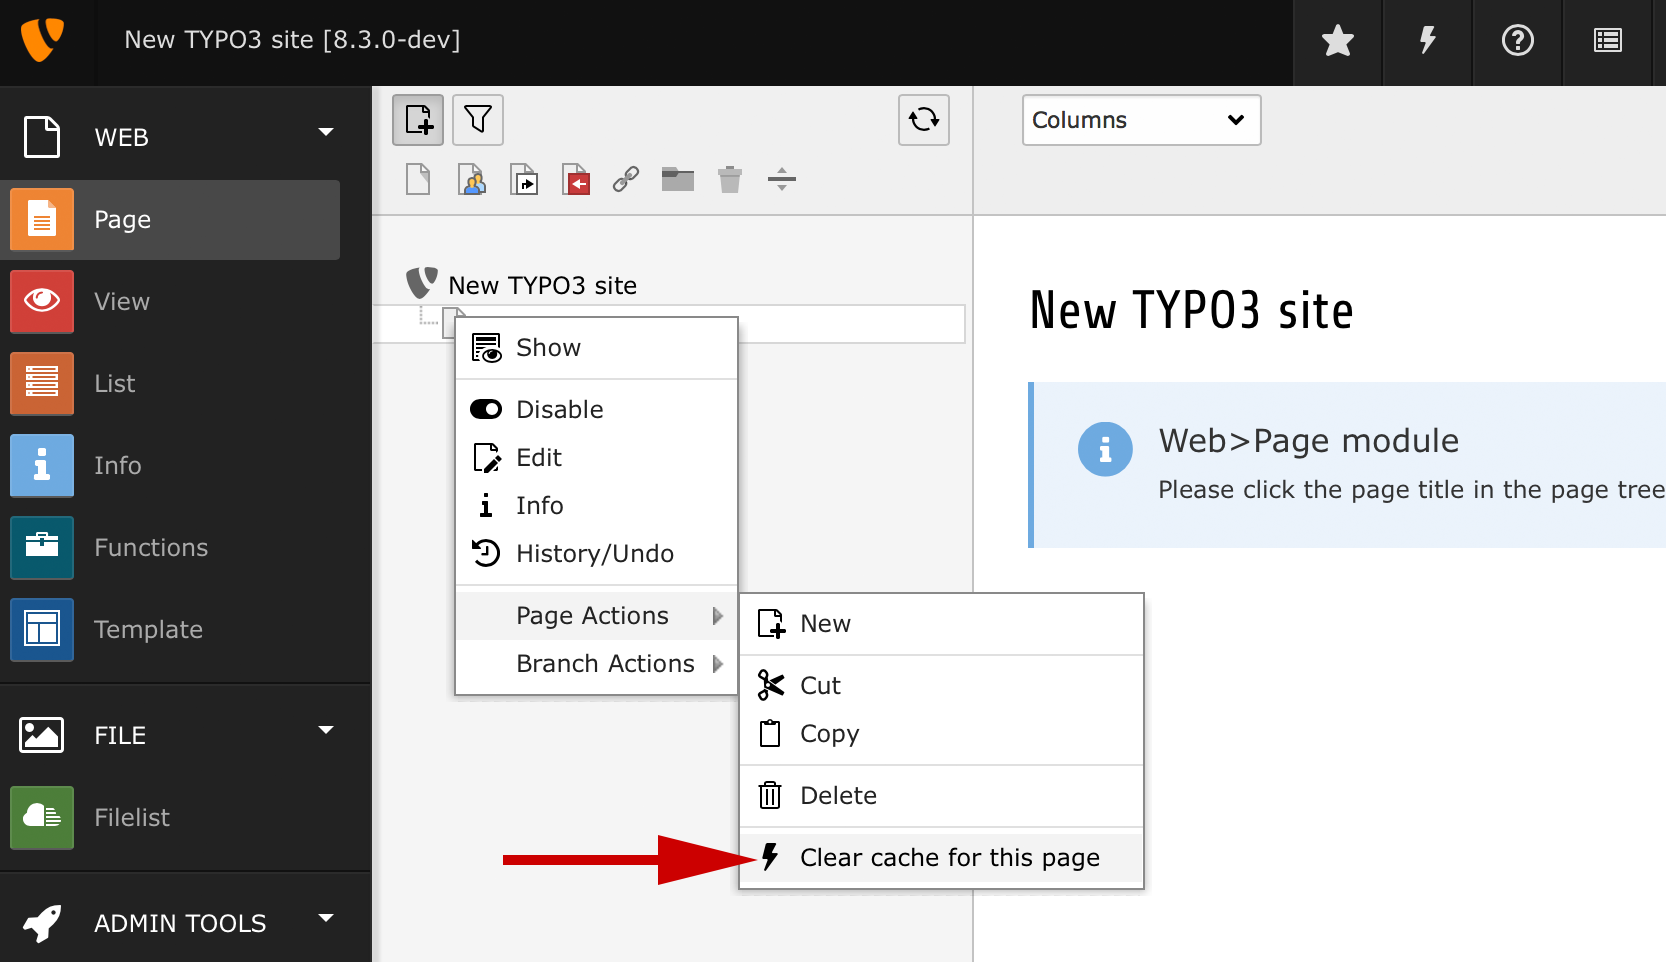
\includegraphics[width=0.70\linewidth]{BackendUserInterface/20446.png}
	\end{figure}

\end{frame}

% ------------------------------------------------------------------------------
% LTXE-SLIDE-START
% LTXE-SLIDE-UID:		8544ef75-dc66f8b5-5b77a2a3-4fe5539b
% LTXE-SLIDE-ORIGIN:	5b0090eb-13043388-8c4dee34-6cac1521 English
% LTXE-SLIDE-TITLE:		!Feature: #76072 - Ogg, flac and opus support
% LTXE-SLIDE-REFERENCE:	!Feature-76072-OggFlacAndOpusSupport.rst
% ------------------------------------------------------------------------------
\begin{frame}[fragile]
	\frametitle{Interface Utilisateur Backend}
	\framesubtitle{Support de Ogg, Flac et Opus}

	Le support des formats ouverts suivants est ajouté au champ Élément de média~:
	\texttt{ogg}, \texttt{flac} et \texttt{opus}

	\begin{figure}
		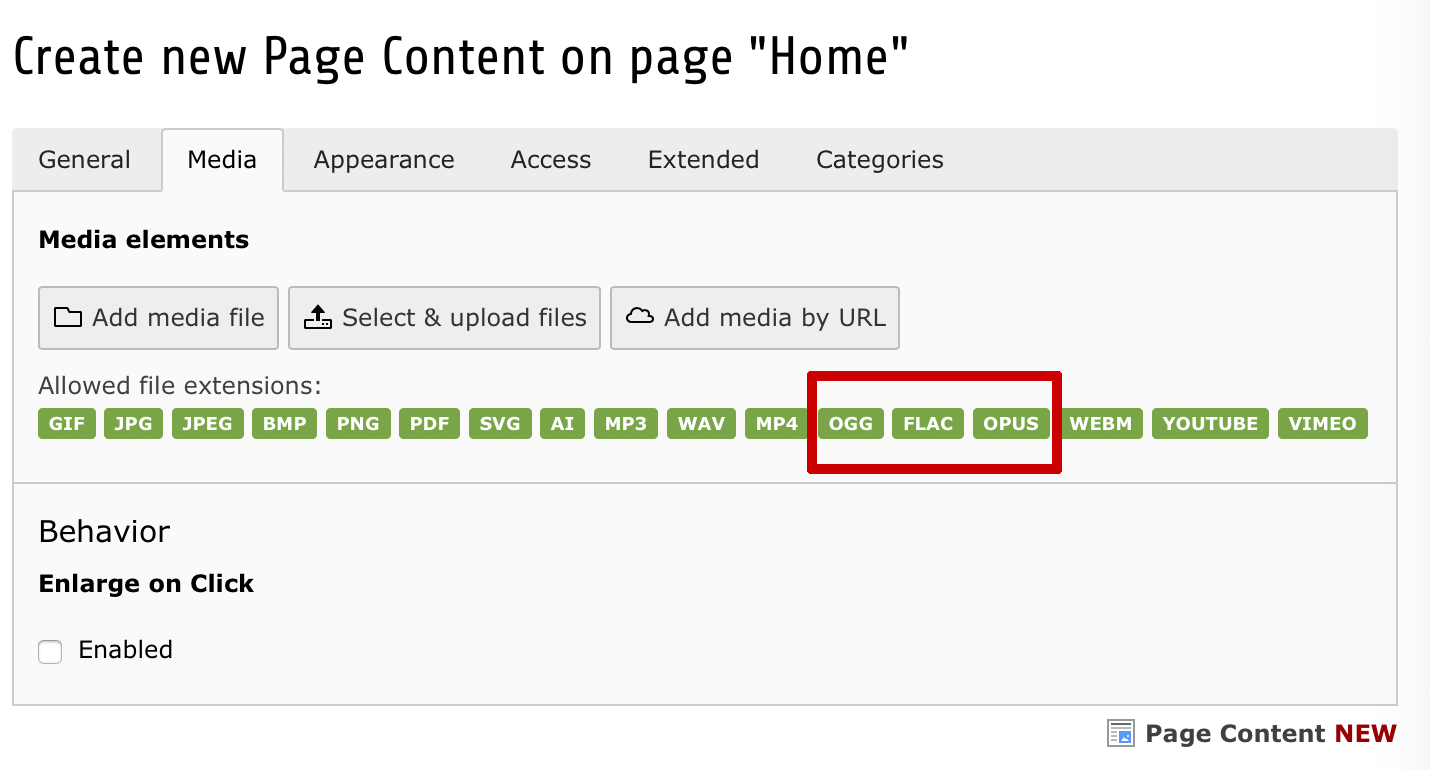
\includegraphics[width=0.70\linewidth]{BackendUserInterface/76072.png}
	\end{figure}

\end{frame}


